\section{Methodology}

\begin{frame}{Project phases}

    The project will be divided into three main phases:

    \begin{enumerate}
        \item \textbf{SIMPLE algorithm:} Implement and test the SIMPLE algorithm to solve the steady-state incompressible Navier-Stokes equations.
        \item \textbf{Velocity field analysis:} Analyze the velocity field around a pillar to determine the optimal position to reduce wind exposure.
        \item \textbf{Report writing:} Summarize the results and findings in a report.
    \end{enumerate}

    Each phase can be further divided into smaller tasks.

\end{frame}



\begin{frame}{Phase 1.1 - SIMPLE Algorithm Implementation}

    \begin{columns}[c, onlytextwidth]

        \begin{column}{0.5\textwidth}

            The SIMPLE algorithm will be implemented in the same codebase used for the implementation of the SCGS algorithm (Assignment 1).

            \vspace{9pt}

            The code will be written in \texttt{C11}.

            \vspace{9pt}

            Only Cartesian equi-spaced grids will be considered for the mesh generation.

        \end{column}

        \begin{column}{0.5\textwidth}

            \begin{figure}
                \centering
                \includegraphics[width=0.9\textwidth]{img/SCGS-screenshot.png}
                \caption{Screenshot of the SCGS codebase.}
            \end{figure}

        \end{column}

    \end{columns}

\end{frame}



\begin{frame}{Phase 1.2 - SIMPLE Algorithm Testing}

    Before proceeding with the velocity field analysis, the SIMPLE algorithm will be tested against the numerical solution of the lid-driven cavity flow provided by \textit{Ghia et al.} \cite{Ghia1982HighReSF}.

    Basically, we will follow the same procedure as in Assignment 1, but using the SIMPLE algorithm instead of the SCGS algorithm.

    \begin{figure}
        \centering
        \includegraphics[width=0.6\textwidth]{img/ghia_solution_Re1000.png}
    \end{figure}

    Once the code is validated, we will proceed with the velocity field analysis.

\end{frame}



\begin{frame}{Phase 2.1 - Square Pillar Modelling}

    At first, we will model a square pillar to analyze the velocity field around it.

    \begin{table}
        \centering
        \begin{tabular}{l|ll}
            Parameter                & Values          & Unit   \\
            \hline
            \textbf{Wind speed}      & $[10, 20]$      & $km/s$ \\
            \textbf{Angle of attack} & $[0, 22.5, 45]$ & $deg$  \\
            \textbf{Pillar size}     & $50$            & $cm$   \\
            \hline
        \end{tabular}
        \caption{Test cases that will be evaluated for the square pillar.}
    \end{table}

    \begin{figure}
        \centering
        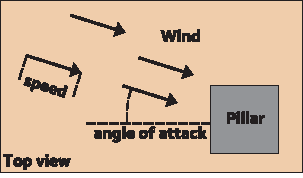
\includegraphics[width=0.5\textwidth]{pdf/Square-pillar.pdf}
    \end{figure}

    At implementation level, we will keep the geometry of the pillar fixed in space and vary the wind speed and angle of attack at the boundary of our computational domain.

\end{frame}



\begin{frame}{Phase 2.2 - Circular Pillar Modelling}

    At second, we will model a circular pillar to analyze the velocity field around it.

    \begin{table}
        \centering
        \begin{tabular}{l|ll}
            Parameter                & Values     & Unit   \\
            \hline
            \textbf{Wind speed}      & $[10, 20]$ & $km/s$ \\
            \textbf{Pillar diameter} & $60$       & $cm$   \\
            \hline
        \end{tabular}
        \caption{Test cases that will be evaluated for the circular pillar.}
    \end{table}

    \begin{figure}
        \centering
        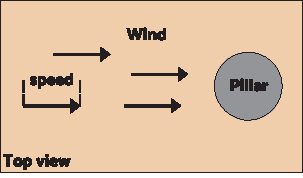
\includegraphics[width=0.5\textwidth]{pdf/Circular-pillar.pdf}
        \hspace{18pt}
        \includegraphics[width=0.3\textwidth]{img/Circular-approximation.png}
    \end{figure}

    At implementation level, since our solver will only implement Cartesian grids, we will approximate the circular shape by a series of rectilinear cells.

\end{frame}



\begin{frame}{Phase 2.3 (optional) - Shelter Modelling}

    Time permitting, we will also model a shelter to analyze the velocity field inside and around it, to understand the effectiveness of such a structure in reducing wind exposure.

    Simulation parameters will be similar to the ones used for the square pillar.

    \begin{figure}
        \centering
        \includegraphics[width=0.7\textwidth]{img/shelter.png}
        \caption{Bus shelter in Columbia St., Waterloo, ON.}
    \end{figure}

\end{frame}



\begin{frame}{Phase 3 - Report Writing}

    Once all the simulations are completed, we will write a report summarizing the results and findings.

    The report we will include:

    \begin{itemize}
        \item Introduction: Briefly introduce the problem and the objectives of the study.
        \item Methodology: Describe the numerical methods used and the test cases considered (focusing on the boundary conditions considered and their implementation at code level).
        \item Results: Present the results of the velocity field analysis.
    \end{itemize}

    In the result section we will try to include a clear visualization of the optimal position depending on the conditions considered (wind speed, angle of attack, and geometry of the pillar).

\end{frame}